\documentclass{article}
\usepackage{color}
\usepackage{graphicx}

\begin{document}
\let\thefootnote\relax\footnotetext{Last edited March 7, 2015 by KO}

\section{Sodium consumption and life expectancy}

Summary of the data preprocessing:
\begin{itemize}
\item We split the data by year, 1990 and 2010, in which the sodium data was recorded. Within each of these datasets, we imputed the missing values for predictors by taking the median for that variable.
\item Sex-specific alcohol consumption measurements were only available in 2010, so we used overall alcohol consumption for 1990. No other predictor was sex-specific. 
\item We removed Chile from the analysis because there was no life expectancy data for 2010. 36 countries remained.
\item	We took the difference between 2010 and 1990 for all (numeric) variables.
\end{itemize}

We tested the hypothesis of association between sodium intake and excess mortality.  In our dataset, ``excess mortality'' is signified by a decrease in life expectancy from 1990 to 2010 beyond what would be expected given the other characteristics of a country.  We measured this by modeling the change in life expectancy using alcohol consumption and per capita GDP.  For our dataset, we fit several predictive models (ordinary linear regression, linear regression with polynomial terms, regression trees, bagged regression trees, random forests, support vector machines, boosted trees, and neural networks).  For each type of model, we tuned the parameters by training on bootstrap samples of the data and choosing the tuning parameter that results in the smallest average prediction error.  Finally, we among these tuned models, we chose the model with the smallest mean squared error.  For males, the model with best fit was a support vector machine with radial basis function kernel, and for females, the model with best fit was a random forest.  The residuals from these model represent the change in life expectancy not explained by alcohol consumption and per capita GDP. \\

We measured the strength of the association between sodium intake and the residuals from the model using Pearson's correlation. We tested the significance of the association using a permutation test.  Under the null hypothesis of no association, the residuals of the model are exchangeable: if sodium intake has no effect on mortality, then the residuals are equally likely to be paired with any of the sodium measurements.  Under the alternative hypothesis, our model will tend to \textit{overestimate} the increase in life expectancy from 1990 to 2010 in countries where sodium intake increased and to \textit{underestimate} the change in life expectancy in countries where sodium intake decreased. This alternative corresponds to a significant positive correlation between the residuals and change in sodium intake.  The correlation for males was $-0.0933$ (one-sided p-value $0.698$, two-sided p-value $0.594$) and the correlation for females was $-0.3302$ (one-sided p-value $0.9768$, two-sided p-value $0.0489$) (Figure~\ref{fig:sodium_excessmortality}). We conclude there is insufficient evidence to reject the null hypothesis that the correlation is $0$.  In fact, the correlation between change in sodium consumption and excess mortality for females is significantly less than $0$; an increase in sodium consumption is associated with a greater change in life expectancy than we would predict, given a country's alcohol consumption and per capita GDP. \\



\begin{figure}
\centering
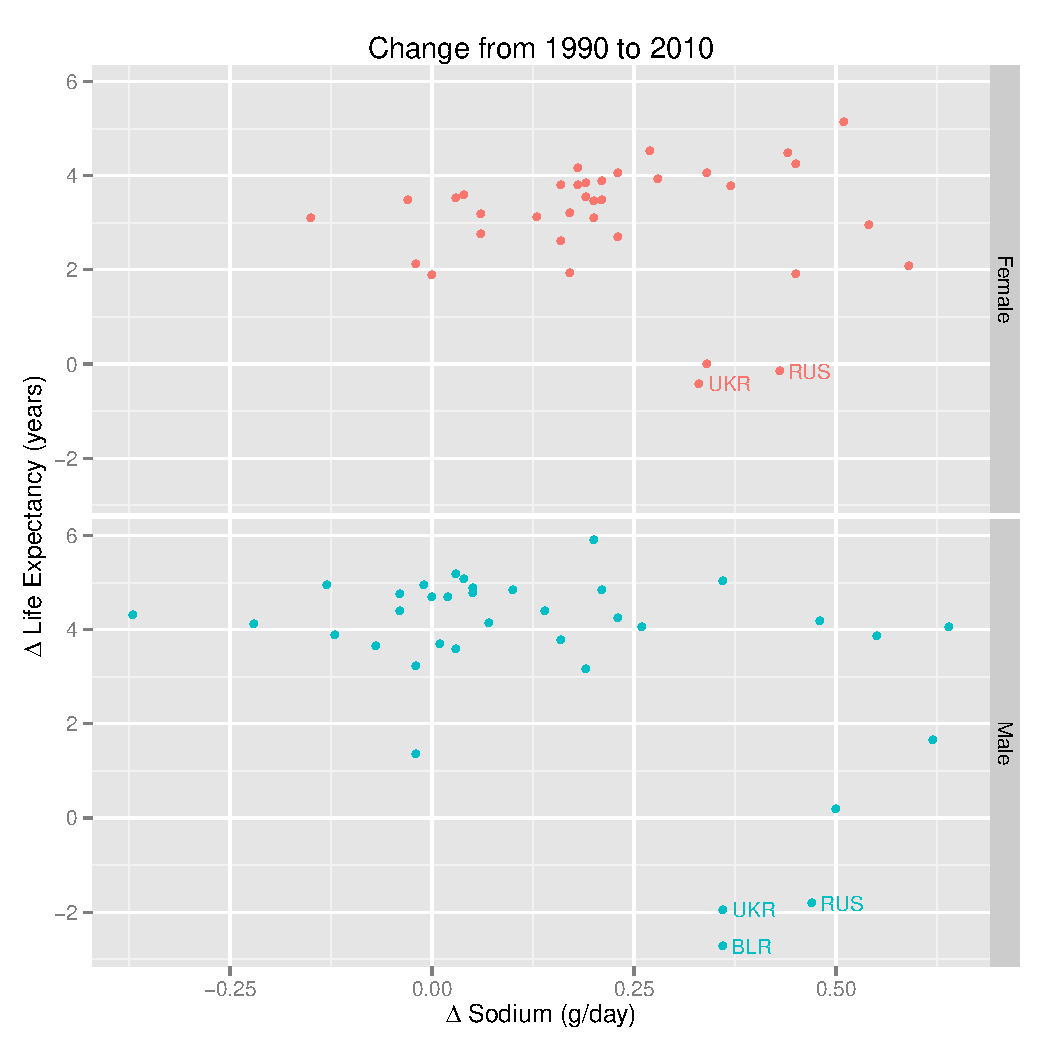
\includegraphics[scale = 0.5]{sodium_lifeexp.pdf}
\caption{Scatterplot of change in sodium intake against change in life expectancy at age 30 from 1990 to 2010. Even before correcting for the effect of other social and economic factors, there is no obvious association between sodium and life expectancy.}\label{fig:sodium_lifeexp}
\end{figure}

\begin{figure}
\centering
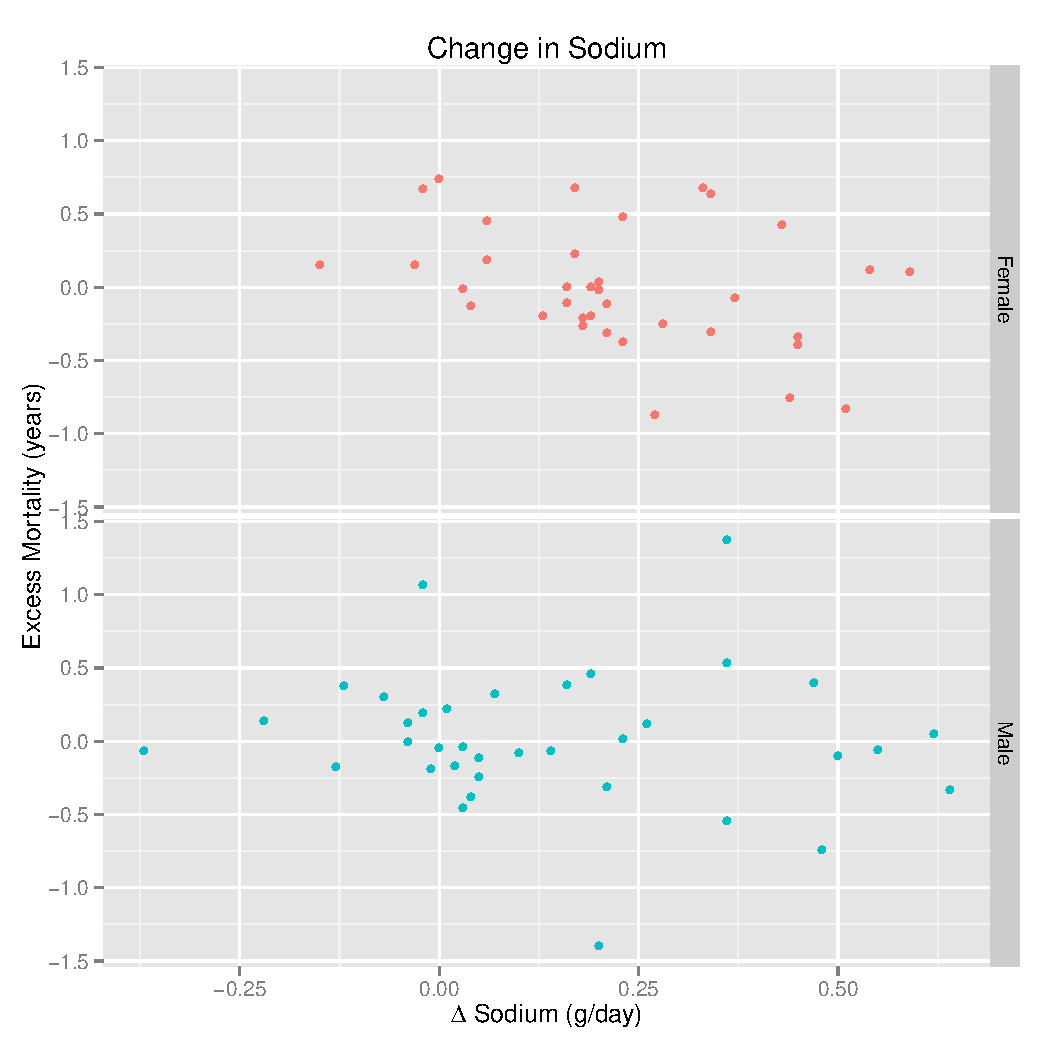
\includegraphics[scale = 0.5]{sodium_exmort.pdf}
\caption{Scatterplot of change in sodium intake against excess mortality.}\label{fig:sodium_excessmortality}
\end{figure}

\section{Smoking and life expectancy}
We repeated the analysis, switching the roles of sodium and cigarettes smoked.  Data preprocessing was identical to that of the first analysis, except...

\end{document}